\item \textbf{{[}JPJC/PRELIM/9597/2019/P1/Q4{]} }

You are to write a computer program to test the validity of classic
Sudoku puzzles. 

The classic Sudoku puzzle involves a grid of 81 squares. The grid
is divided into nine blocks, each containing nine squares. Each of
the nine blocks has to contain all the numbers 1 to 9 within its squares.
Each number can only appear once in a row, column or block. 

A $9\times9$ classic Sudoku puzzle can be represented using a two-dimensional
array. An example of this puzzle is:
\begin{center}
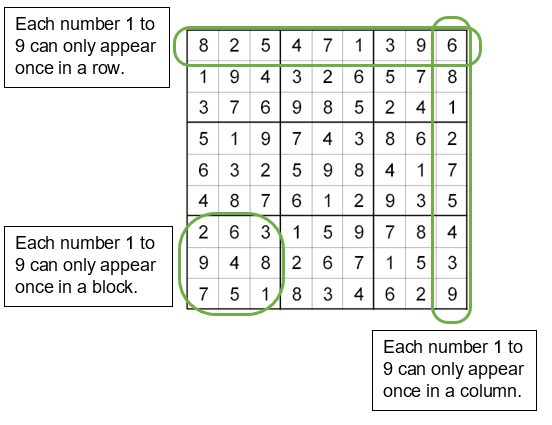
\includegraphics[width=0.5\paperwidth]{C:/Users/Admin/Desktop/Github/question_bank/LyX/static/img/9597-JPJC-2019-P1-Q4-1}
\par\end{center}

The puzzle can be displayed in this way on the computer. 
\noindent \begin{center}
\texttt{}%
\begin{tabular}{c}
\texttt{8 2 5 4 7 1 3 9 6}\tabularnewline
\texttt{1 9 4 3 2 6 5 7 8}\tabularnewline
\texttt{3 7 6 9 8 5 2 4 1}\tabularnewline
\texttt{5 1 9 7 4 3 8 6 2}\tabularnewline
\texttt{6 3 2 5 9 8 4 1 7}\tabularnewline
\texttt{4 8 7 6 1 2 9 3 5}\tabularnewline
\texttt{2 6 3 1 5 9 7 8 4}\tabularnewline
\texttt{9 4 8 2 6 7 1 5 3}\tabularnewline
\texttt{7 5 1 8 3 4 6 2 9}\tabularnewline
\end{tabular}
\par\end{center}

\noindent \begin{center}
\par\end{center}

\subsection*{Task 4.1 }

Write program code for a procedure \texttt{displayboard} that will
take a parameter \texttt{board} and display a puzzle declared as a
two-dimensional array. 

Copy and paste array \texttt{puzzle1} from the file \texttt{PUZZLES.txt}
into your program code. 

Call procedure \texttt{displayboard} to display \texttt{puzzle1}. 

\subsection*{Evidence 11: }
\begin{itemize}
\item Your program code for \texttt{displayboard} to display \texttt{puzzle1}. 
\item Screenshot of displaying \texttt{puzzle1} as a $9\times9$ Sudoku
puzzle.\hfill{} {[}5{]} 
\end{itemize}
To test the validity of a Sudoku puzzle, each of the rows, columns
and blocks can be checked to ensure that each number 1 to 9 only appears
once. 

\subsection*{Task 4.2 }

Write program code for a function \texttt{checkRow} that will check
all the nine rows of the puzzle to ensure that each number 1 to 9
only appears once. The function should take a parameter board and
return a Boolean value. 

\subsection*{Evidence 12: }

Your program code for \texttt{checkRow}.\hfill{} {[}6{]}

\subsection*{Task 4.3}

Write program code for a function \texttt{checkColumn} that will check
all the nine columns of the puzzle to ensure that each number 1 to
9 only appears once. The function should take a parameter \texttt{board}
and return a Boolean value.

\subsection*{Evidence 13: }

Your program code for \texttt{checkColumn}. \hfill{}{[}6{]}

\section*{Task 4.4 }

Write program code for a function \texttt{checkBlock} that will check
all the nine blocks of the puzzle to ensure that each number 1 to
9 only appear once. The function should take a parameter board and
return a Boolean value. 

\subsection*{Evidence 14: }

Your program code for \texttt{checkBlock}.\hfill{} {[}8{]}

\subsection*{Task 4.5 }

Write program code to call the three functions \texttt{checkrow},
\texttt{checkColumn}, and \texttt{checkBlock} to test the validity
of \texttt{puzzle1}, \texttt{puzzle2}, and \texttt{puzzle3} given
in the file \texttt{PUZZLES.txt}. Copy and paste these puzzles into
your program code. Your program should first display the puzzle before
printing statement(s) to show whether the puzzle is valid or not.
If invalid, state whether the invalidity is due to the row, column
or block.

\subsection*{Evidence 15:}

\textbullet{} Your program code for task 4.5 

\textbullet{} Screenshot of running task 4.5\hfill{} {[}5{]}